% Created 2020-10-01 Thu 16:05
% Intended LaTeX compiler: pdflatex
\documentclass[10pt,t]{beamer}
\usepackage[utf8]{inputenc}
\usepackage[T1]{fontenc}
\usepackage{graphicx}
\usepackage{grffile}
\usepackage{longtable}
\usepackage{wrapfig}
\usepackage{rotating}
\usepackage{amsmath}
\usepackage{textcomp}
\usepackage{amssymb}
\usepackage{capt-of}
\usepackage{hyperref}
\usetheme{default}
\author{L. Larrabee Strow}
\date{\today}
\title{\large AIRS/CrIS Radiometricc Stability Improvements Needed for the CHIRP Climate Data Record}
\subtitle{\footnotesize{AIRS Virtual Science Team Meeting}}
\date{\vspace{0.1in}\footnotesize{May 12, 2019 \vfill}}
\author{L. Larrabee Strow\inst{1,2}, Andy Tangborn \inst{2}, and Howard Motteler\inst{2} }
\institute[UMBC]{\inst{1} UMBC Physics Dept. \and \inst{2}UMBC JCET}
\input beamer_setup
\usetheme{metropolis}
\metroset{titleformat title=allcaps}
\renewcommand{\UrlFont}{\small\tt}
\renewcommand*{\UrlFont}{\footnotesize}
\tolerance=1000
\begin{document}

\maketitle


\begin{frame}[label={sec:org395e072}]{Introduction}
Something
\end{frame}

\begin{frame}[label={sec:org1248642}]{AIRS Radiometric Drifts via DCC's}
\vspace{-0.4in}
\begin{columns}
\begin{column}{0.5\columnwidth}
\begin{block}{\scriptsize Mean DCC Spectrum}
\vspace{-0.12in}
\begin{center}
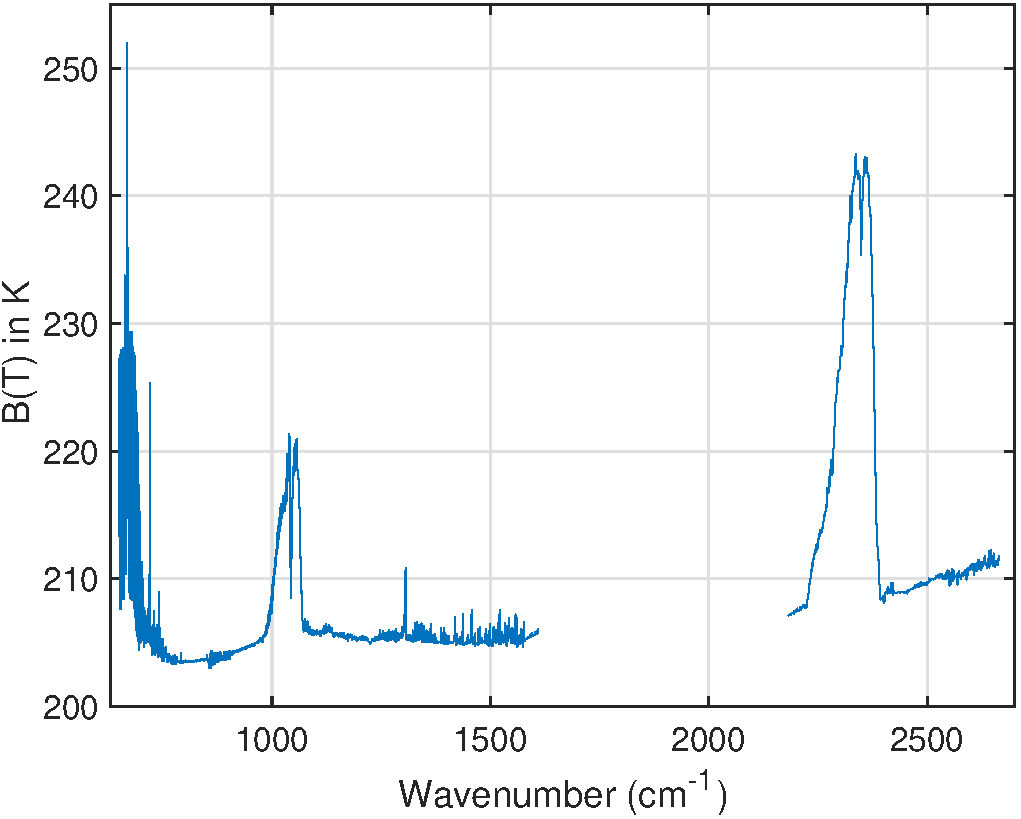
\includegraphics[width=0.95\linewidth]{./Figs/Pdf/mean_dcc_spectrum.pdf}
\end{center}
\end{block}
\end{column}

\begin{column}{0.5\columnwidth}
\begin{block}{\scriptsize 15-Year DCC Trend}
\vspace{-0.12in}
\begin{center}
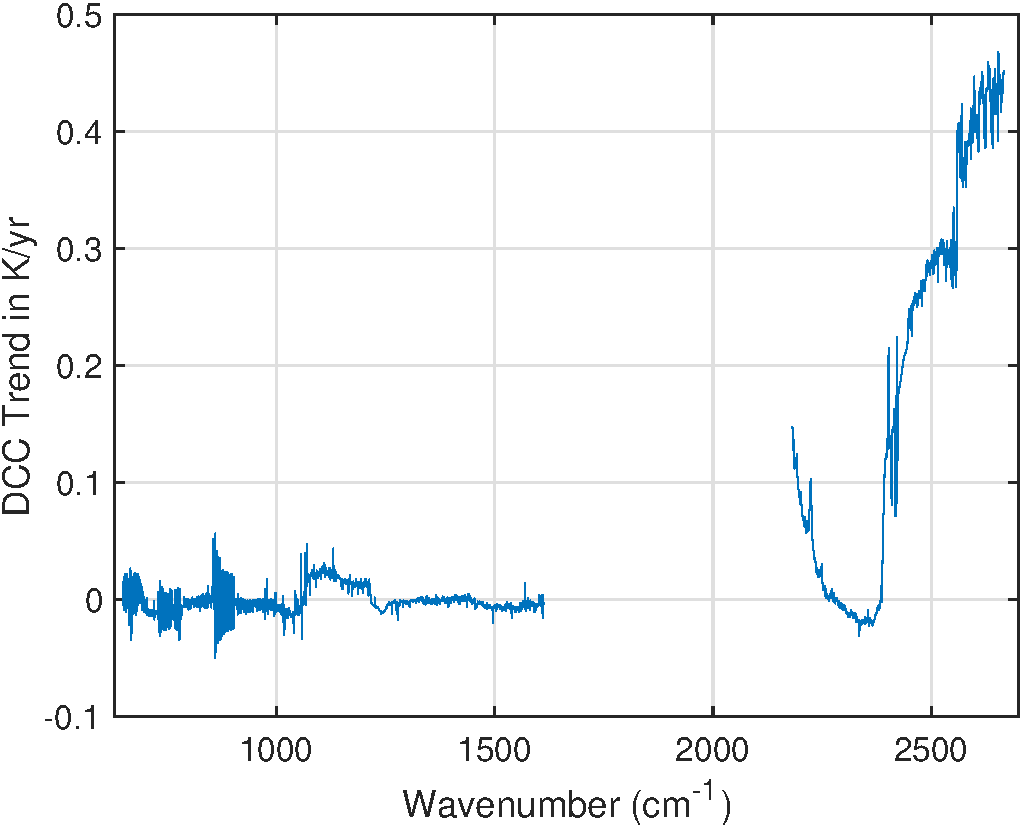
\includegraphics[width=0.95\linewidth]{./Figs/Pdf/dcc_trend.pdf}
\end{center}
\end{block}
\end{column}
\end{columns}

\vspace{-0.25in}
\begin{columns}
\begin{column}{0.5\columnwidth}
\begin{block}{\scriptsize Time Dependence of Trends}
\vspace{-0.12in}
\begin{center}
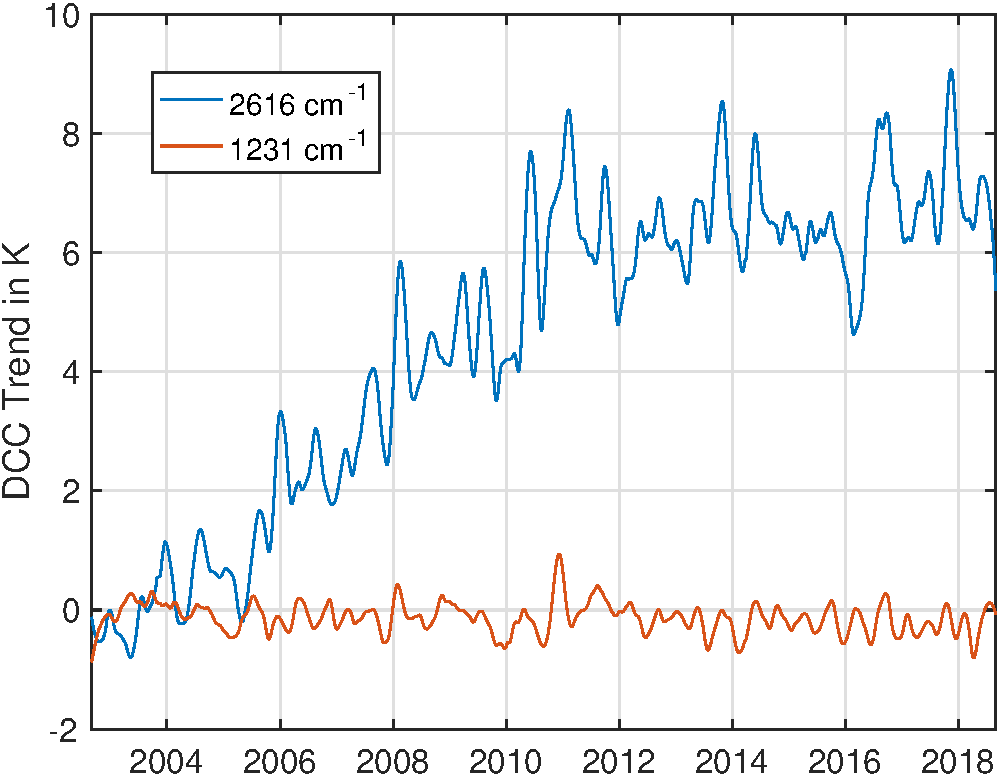
\includegraphics[width=0.8\linewidth]{./Figs/Pdf/dcc_drift_vs_time_1231_2616.pdf}
\end{center}
\end{block}
\end{column}

\begin{column}{0.58\columnwidth}
\begin{block}{}
\vspace{-0.15in}
\scriptsize
\begin{itemize}
\item DCC's defined here by BT(960 \wn) < 215K
\item DCC's often used for calibration since extremely stable
\item Trends are NOT seen in IASI shortwave
\item A/B trends (longwave) and AIRS frequency shifts have similar time-dependencies!
\item Shortwave sensitive to space view (SV) drifts.
\item Suspect focal plane/optics shifts that change location of SV's
\end{itemize}
\end{block}
\end{column}
\end{columns}
\end{frame}

\begin{frame}[label={sec:orgd21ecfb},shrink=20]{Using DCC Emission to Determine Calibration Drifts}
\begin{itemize}
\item Simplified to ignore non-linearity and polarization
\item Written differently than in ATBD, show Space View (SV) explicitely
\end{itemize}

\vspace{-0.2in}

\begin{columns}
\begin{column}{0.3\columnwidth}
\begin{block}{}
\vspace{-0.12in}
\begin{equation}
R = \frac{EV - SV}{OBC - SV} R_{\text OBC}
\nonumber
\end{equation}
\end{block}
\end{column}

\begin{column}{0.9\columnwidth}
\begin{block}{}
\vspace{-0.12in}
\begin{itemize}
\item R is calibrated radiance
\item EV/SV/OBC are the earth/space/blackbody counts
\item R\textsubscript{\text{OBC}} is the computed OBC (blackbody) radiance
\end{itemize}
\end{block}
\end{column}
\end{columns}



\begin{columns}
\begin{column}{0.55\columnwidth}
\begin{block}{Sensitivity of R to SV}
\vspace{0.1in}
\begin{equation}
\frac{\partial R}{\partial SV} = \frac{1}{OBC - SV} (R - R_{\text{OBC}})
\nonumber
\end{equation}
\end{block}
\end{column}

\begin{column}{0.55\columnwidth}
\begin{block}{Solve for SV}
\vspace{0.1in}
\begin{equation}
\delta SV = \frac{OBC - SV}{R - R_{\text{OBC}}} \delta R
\nonumber
\end{equation}
\end{block}
\end{column}
\end{columns}





\begin{block}{Approach}
\begin{itemize}
\item Use DCC trends for \(\delta\) R, solve for \(\delta\) SV (\(\equiv\) SV drift/year)
\item Compute \(\delta\) R trends for various scene types (R = DCC, clear, etc.)
\item Convert to BT trends
\item Ignore regions where emission exists above DCC's, ie stratospheric emission that could be varying in time
\item Lien \#1: used a single, randomly selected AIRS L1a scene to estimate (OBC - SV)
\item Lien \#2: DCC drift maximum near equator, drops 30\% by \textpm{} 30\textdegree{} latitude (orbit phase or T. Pagano's FOV idea?)
\end{itemize}
\end{block}
\end{frame}

\begin{frame}[label={sec:org70b8f99}]{SV Trend Results}
\vspace{-0.4in}

\begin{columns}
\begin{column}{0.5\columnwidth}
\begin{block}{\scriptsize Sample Set of AIRS L1a Counts}
\vspace{-0.12in}
\begin{center}
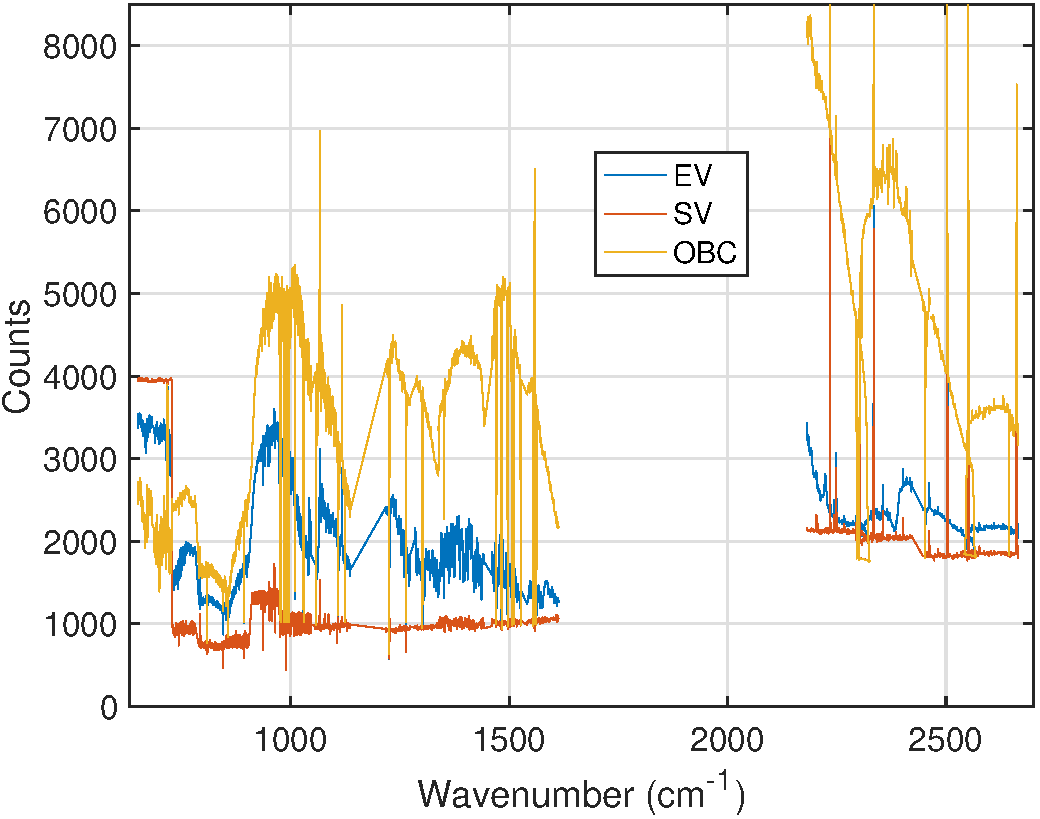
\includegraphics[width=0.95\linewidth]{./Figs/Pdf/airs_counts_example.pdf}
\end{center}
\end{block}
\end{column}

\begin{column}{0.5\columnwidth}
\begin{block}{\scriptsize \(\delta\) BT for 1\% SV drift for BT = DCC, 300K}
\vspace{-0.12in}
\begin{center}
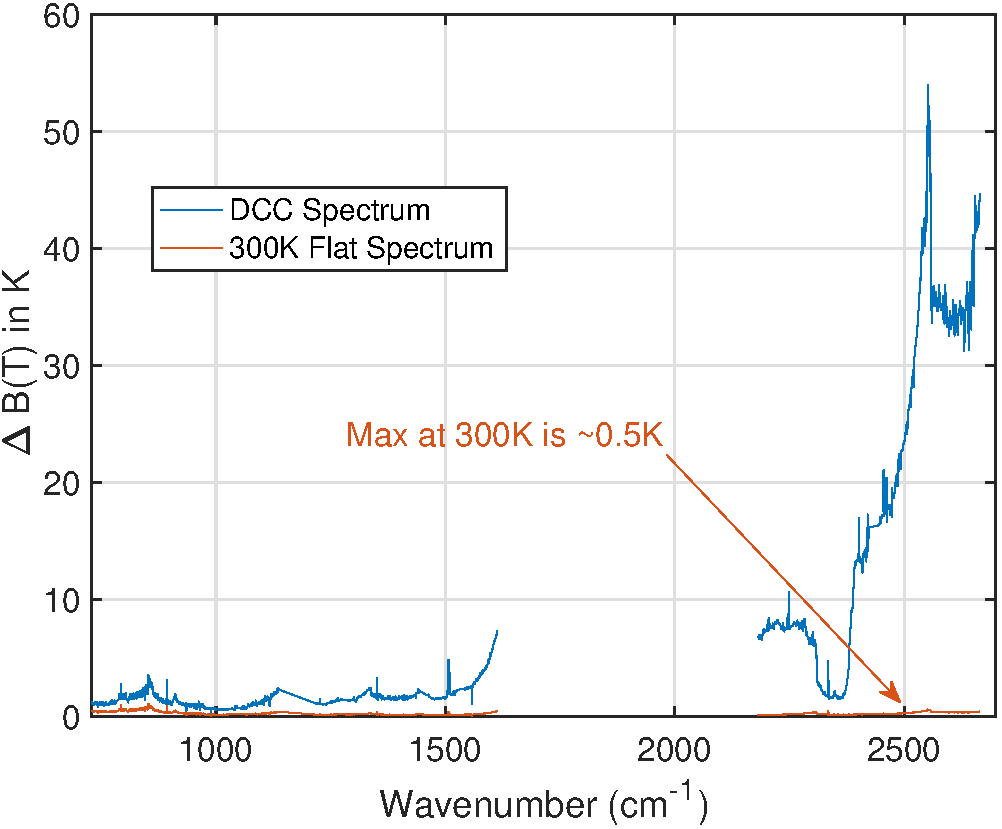
\includegraphics[width=0.93\linewidth]{./Figs/Pdf/dbt_for_minus1pc_dsv_for_dcc_spectrum_and_300k.pdf}
\end{center}
\end{block}
\end{column}
\end{columns}


\vspace{-0.25in}
\begin{columns}
\begin{column}{0.5\columnwidth}
\begin{block}{\scriptsize \(\delta\) SV BT Trend for SV = 265K}
\vspace{-0.12in}
\begin{center}
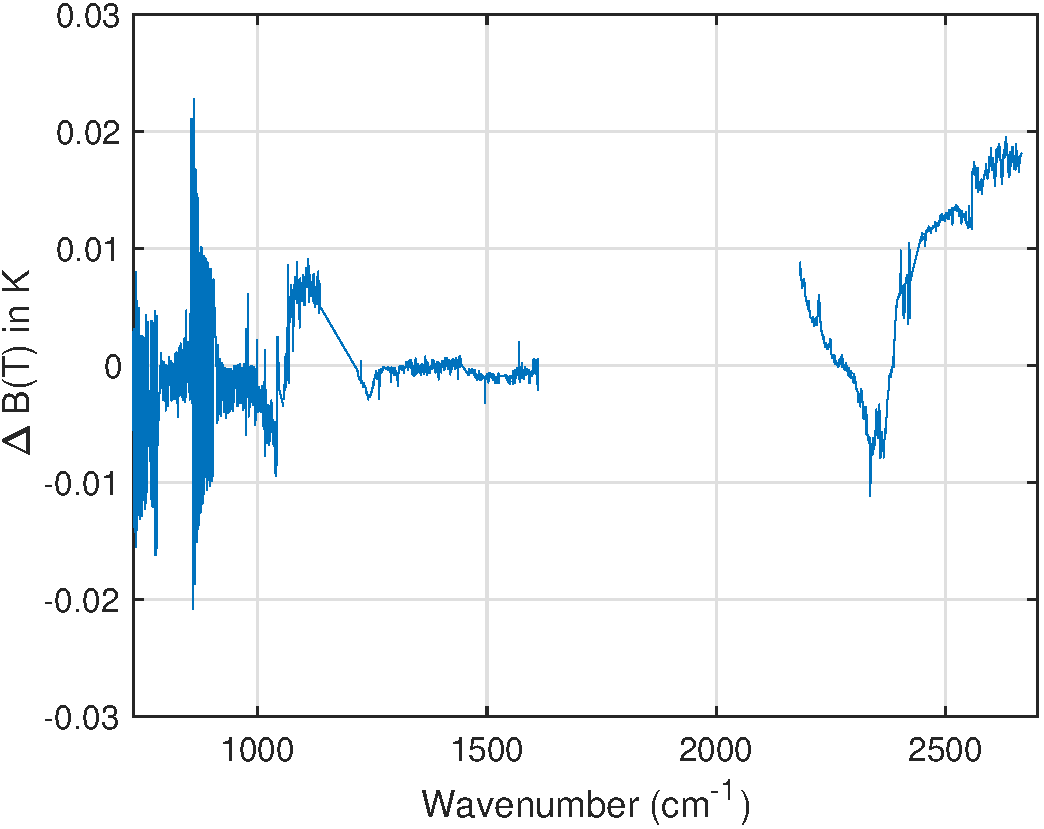
\includegraphics[width=0.8\linewidth]{./Figs/Pdf/dbt_sv_if_sbt_is_265k.pdf}
\end{center}
\end{block}
\end{column}

\begin{column}{0.55\columnwidth}
\begin{block}{}
\vspace{-0.15in}
\scriptsize
\begin{itemize}
\item AIRS scene produces window BT \textasciitilde{}275K
\item Note high A/B variability in SV counts!
\item Setting SV = 265K is just to illustrate magitude of SV drift
\item SV drifts \emph{small} but DCC's allow quantification
\item Key conclusion: this approach predicts scene dependence
\end{itemize}
\end{block}
\end{column}
\end{columns}
\end{frame}

\begin{frame}[label={sec:org0628e38}]{Do the DCC SV Drifts Predict All-Sky Trends?}
\vspace{-0.1in}
\begin{center}
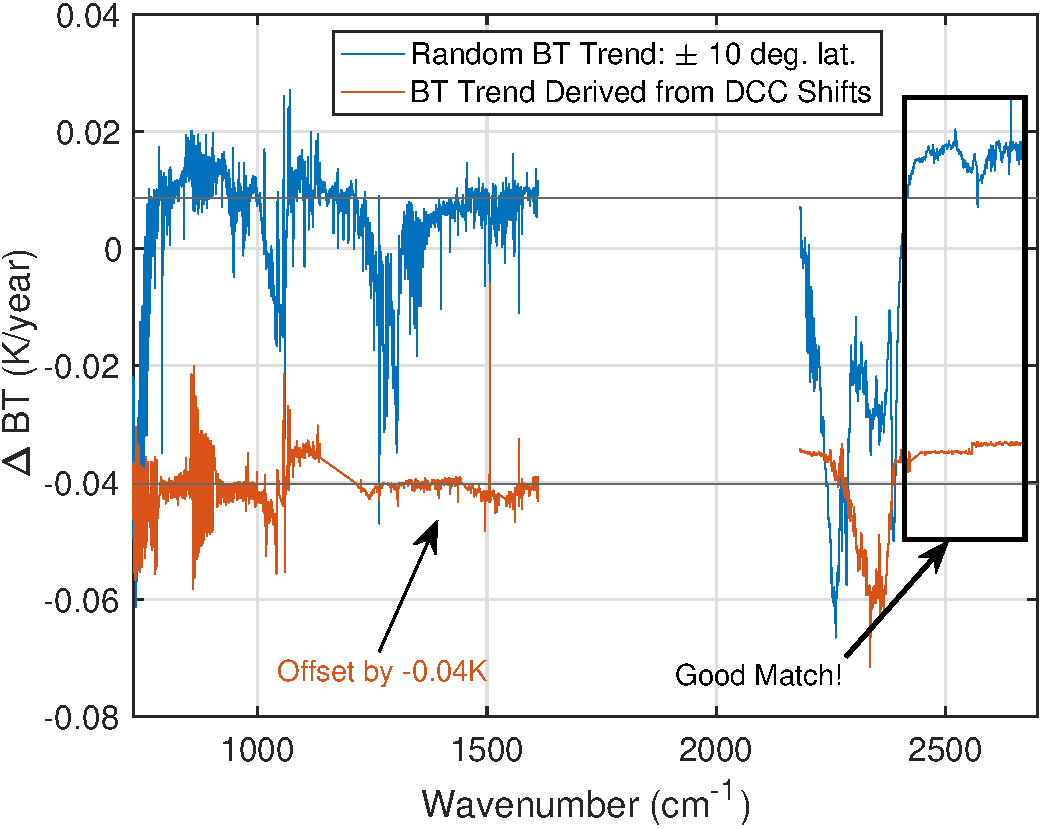
\includegraphics[width=0.65\linewidth]{./Figs/Pdf/random_trend_with_drift_for_that_bt_from_dcc_drifts.pdf}
\end{center}

\vspace{-0.1in}

\scriptsize
\begin{itemize}
\item Blue is 17-year all-sky AIRS BT trend (black line denotes 1231 \wn channel)
\begin{itemize}
\item \scriptsize \cd, \methane, \nitrous, and \ozone exhibit greenhouse effect
\item \scriptsize \water also shows greenhouse effect
\end{itemize}
\item Red are shifts predicted by SV drift.  Nicely reproduces shortwave "false" extra warming
\item Nominal agreement for detector side A/B ringing in window regions
\item LIEN: SV trend likely orbit phase dependent!
\end{itemize}
\end{frame}
\end{document}